\documentclass[aspectratio=1610,t]{beamer}

% Colors
\usepackage{color}
\definecolor{mainorange}{HTML}{EC811B}
\definecolor{lightgrey}{HTML}{888888}

% Syntax highlighting
\usepackage{minted}
\usepackage{alltt}
\newcommand\hi[1]{{\color{mainorange} \textbf{#1}}}

% Theme
\usetheme[%
	subsectionpage=progressbar,
	numbering=fraction,
	progressbar=foot,
]{metropolis}

% Customization
\setbeamertemplate{section in toc}[sections numbered]
\setbeamerfont{title}{size=\fontsize{30}{30}}
\setbeamerfont{block title}{size=\large}
\newcommand\sep{\textcolor{lightgrey}{\rule{\linewidth}{0.05mm}}}

% Meta
\title{Parallel Programming with Thread pools and iterators}
\date{\today}
\author{Stefan Schindler (@dns2utf8)}
\institute{Rust Zürichsee, Schweiz, CH - hosted by Cloud Solutions Amsterdam, NL}

\begin{document}

\pgfdeclareimage[width=\paperwidth]{bg}{background-light.pdf}
\pgfdeclareimage[width=\paperwidth]{bgdark}{background-dark.pdf}

\usebackgroundtemplate{\pgfuseimage{bgdark}}
\maketitle

% ----------------------------------------------------------------- %

\begin{frame}[plain,noframenumbering]
	\frametitle{Index}
	\setcounter{tocdepth}{1}
	\tableofcontents
\end{frame}

% ----------------------------------------------------------------- %

\usebackgroundtemplate{\pgfuseimage{bg}}

{
\usebackgroundtemplate{\pgfuseimage{bgdark}}
\section{About me}
}

\begin{frame}[fragile]{Timetable}
  \begin{itemize}
    \item 18:30 => Venue opens, pizza's arrive
    \item now => Talk Stefan: Parallel Programming with Rust
    \item 19:30 => Break
    \item 19:45 => Maarten: How to speed up your builds with Bazel
    \item 20:15 => Discussions
    \item 21:00 => Venue closes
    \item tomorrow => ???
    \item the day after => parallelize the World!
  \end{itemize}
\end{frame}
% timetable


\begin{frame}[fragile]{About:me}
Hello my name is Stefan and I work on and with computers.

I organize
\begin{itemize}
  \item RustFest.eu Next: probably in September 2019 with "impl days" before or after the conference
  \item Meetups in and around Zürich, CH
  \item ErnstEisprung.ch (in de Zwitserse Alpen Juli 2019)
\end{itemize}

Some of my side projects
\begin{itemize}
  \item rust threadpool (maintainer)
  \item Son of Grid Engine (SGE) interface
  \item run your own infrastructure - DNS, VPN, Web, ...
\end{itemize}
\end{frame}



\begin{frame}[fragile]{What will we learn tonight?}

\begin{itemize}
 \item Loops
 \item Iterators
 \item Different modes of execution
 \item Single vs. Multi Threading
 \item How to synchronize pools
 \item Hot to translate linear into parallel code
\end{itemize}

\end{frame}

{
\usebackgroundtemplate{\pgfuseimage{bgdark}}
\section{Loops}
}

\begin{frame}[fragile]{Loops 0 - What happened so far}
\begin{minted}{C}
const char *data[] = { "Peter Arbeitsloser", ... };

  const int length = sizeof(data) / sizeof(data[0]);
  int index = 0;
head:
  if (!(index < length)) {
    goto end;
  }
  const char *name = data[index];
  printf("%i: %s\n", index, name);
  index += 1;
  goto head;
end:
\end{minted}
\end{frame}

\begin{frame}[fragile]{Loops 1 - What improved}
\begin{minted}{C}
const char *data[] = {
    "Peter Arbeitsloser",
    "Sandra Systemadministratorin",
    "Peter Koch",
};

  const int length = sizeof(data) / sizeof(data[0]);

  for (int index = 0; index < length; ++index) {
    const char *name = data[index];
    printf("%i: %s\n", index, name);
  }
\end{minted}
\end{frame}

\begin{frame}[fragile]{Loops 2 - What happens in rust}
For the following slides keep this in mind:

\begin{minted}{rust}
#[allow(non_upper_case_globals)]
const data: [&str; 3] = [
    "Peter Arbeitsloser",
    "Sandra Systemadministratorin",
    "Peter Koch",
];
\end{minted}
\end{frame}

\begin{frame}[fragile]{Loops 3 - While}
\begin{minted}{rust}
    let mut index = 0;
    let length = data.len();
    while index < length {
        println!("{}: {}", index, data[index]);
        index += 1
    }
\end{minted}
\end{frame}

\begin{frame}[fragile]{Loops 4 - For each}
\begin{minted}{rust}
    for name in &data {
        println!("{}", name);
    }
\end{minted}

Note the \textbf{\&} next to \texttt{data}.
\end{frame}

\begin{frame}[fragile]{Loops 5 - Iterator}
\begin{minted}{rust}
    for name in data.iter() {
        println!("{}", name);
    }
\end{minted}

If we prefer a more functional style:
\begin{minted}{rust}
    let iterator = data.iter();
    iterator.for_each(|name| {
        println!("{}", name);
    });
\end{minted}
\end{frame}


{
\usebackgroundtemplate{\pgfuseimage{bgdark}}
\section{Iterators}
}

\begin{frame}[fragile]{Trait Iterator}
\begin{minted}{rust}
    // std::iter::Iterator
    pub trait Iterator {
        type Item;
        fn next(&mut self) -> Option<Self::Item>;
    }

    // For reference std::option::Option
    pub enum Option<T> {
        None,
        Some(T),
    }
\end{minted}
\end{frame}

\begin{frame}[fragile]{Iterators 0}
\begin{minted}{rust}
    let iterator = data.iter();
    iterator.for_each(|name| {
        println!("{}", name);
    });
\end{minted}

\begin{itemize}
 \item Why?
 \item Pros for
    \begin{itemize}
     \item People programming (filters, maps, maintainability, ...)
     \item Compiler (optimizations, early returns, edge cases, ...)
    \end{itemize}
\end{itemize}

\textbf{Video (32min):} RustFest Rome 2018 - Pascal Hertleif: Declarative programming in Rust
\begin{itemize}
  \item \href{https://media.ccc.de/v/rustfest-rome-5-declarative-programming-in-rust}{media.ccc.de/v/rustfest-rome-5-declarative-programming-in-rust}
  \item \href{https://www.youtube.com/watch?v=0W20GPEqbcU}{youtube.com/watch?v=0W20GPEqbcU}
\end{itemize}

\end{frame}



\begin{frame}[fragile]{Iterators 1 - Parsing without panic}
\begin{minted}{rust}
struct Person { first_name: String, surname: String, }
let processed = data
        .iter()
        .map(|name| {
            let mut split = name.split(" ");
let (first_name, surname) = (split.next(), split.next());
if first_name.is_none() || surname.is_none() {
    return Err("Unable to parse: to few parts")
}
            Ok(Person {
                first_name: first_name.unwrap().into(),
                surname: surname.unwrap().into(),
            })
        })
        .collect::<Result<Vec<_>, _>>();
\end{minted}
\end{frame}


\begin{frame}[fragile]{Iterators 2 - Parsing without panic}
\begin{minted}{rust}
struct Person { first_name: String, surname: String, }
let processed = data.iter()
        .map(|name| {
            let mut split = name.split(" ");
let (first_name, surname) = (split.next(), split.next());
match (first_name, surname) {
    (Some(first_name), Some(surname)) => {
        Ok(Person {
            first_name: first_name.into(), surname: surname.into(),
        })
    }
    _ => { Err("Unable to parse: to few parts") }
}
        })
        .collect::<Result<Vec<_>, _>>(); // <- magic happened
\end{minted}
\end{frame}



\begin{frame}[fragile]{Iterators 3 - "processed: \{:\#?\}"}
\begin{minted}{rust}
processed: Ok(
    [
        Person {
            first_name: "Peter",
            surname: "Arbeitsloser"
        },
        Person {
            first_name: "Sandra",
            surname: "Systemadministratorin"
        },
        Person {
            first_name: "Peter",
            surname: "Koch"
        }
    ]
)
\end{minted}
\end{frame}



{
\usebackgroundtemplate{\pgfuseimage{bgdark}}
\section{Modes of Execution}
}

\begin{frame}[fragile]{Programming is ...}
... about solving problems

Examples:
\begin{itemize}
  \item Copy data
  \item Enhance audio
  \item Distribute messages
  \item Store data
  \item Prepare thumbnails
\end{itemize}

Key is understanding the problem
\end{frame}

\begin{frame}[fragile]{Single thread - Linear Execution}
How to do more than one thing at the time?

\begin{itemize}
  \item Linear if tasks are short enough
  \item Polling
  \item Event driven (select/epoll or interrupt)
  \item Hardware SIMD
\end{itemize}
\end{frame}

\begin{frame}[fragile]{Simultaneous Multi Threading - SMP}
Let's add another level of abstraction
\begin{itemize}
  \item spawn / join: handle lists of JoinHandles
  \item pools \begin{itemize}
      \item job queue (threadpool)
      \item Work stealing (rayon)
      \item futures (tokio or async/await)
    \end{itemize}
\end{itemize}

New problems: synchronization and communication

\end{frame}

{
\usebackgroundtemplate{\pgfuseimage{bgdark}}
\section{Implementation}
}

\begin{frame}[fragile]{Send and Sync}
Rusts "pick three" (safety, speed, concurrency)

\begin{minted}{rust}
Trait std::marker::Send
\end{minted}
Types that can be transferred across thread boundaries.

\begin{minted}{rust}
Trait std::marker::Sync
\end{minted}
Types for which it is safe to share references between threads.

\end{frame}

\begin{frame}[fragile]{Crates}
Let's reuse that level of abstraction
\begin{itemize}
  \item std::thread::{spawn, join}
  \item pools \begin{itemize}
      \item ThreadPool (Job Queue)
      \item FuturesThreadPool (Work stealing)
    \end{itemize}
  \item rayon (Work stealing)
  \item timely dataflow (distributed actor model)
\end{itemize}

New problems: synchronization and communication

\end{frame}

\begin{frame}[fragile]{Channel example}
\begin{minted}{rust}
use threadpool::ThreadPool; use std::sync::mpsc::channel;
let n_workers = 4; let n_jobs = 8;

let pool = ThreadPool::new(n_workers);
let (tx, rx) = channel();
for _ in 0..n_jobs {
    let tx = tx.clone();
    pool.execute(move || {
        tx.send(1).expect("channel will be there");
    });
}
drop(tx); // <- Why?

assert_eq!(rx.iter() /*.take(n_jobs)*/ .sum()
    , /* n_jobs = */ 8);
\end{minted}
\end{frame}

\begin{frame}[fragile]{Channel cascade example}
\begin{minted}{rust}
let (tx, mut rx) = channel();
tx.send( (0, 0) ).is_ok();
for _ in 0..TEST_TASKS {
    let rx_pre = rx;
    let (tx_chain, rx_chain) = channel();
    rx = rx_chain;

    pool.execute(move || {
        let r = pi_approx_random(TRIES as u64
                                , rand::random::<f64>);
        let b = rx_pre.recv().unwrap();
        tx_chain.send( (b.0 + r.0, b.1 + r.1) ).is_ok();
    });
}
println!("chain.pi: {}", format_pi_approx(rx.recv().unwrap()));
\end{minted}
\end{frame}



{
\usebackgroundtemplate{\pgfuseimage{bgdark}}
\section{Receipt: from Loops to Iterators}
}
\begin{frame}[fragile]{Collect from Channel - 0}
\texttt{v\_len} holds the number of elements we expect
\begin{minted}{rust}
  let mut pictures = vec![];

  for _ in 0..v_len {
    if let Some(pi) = rx.recv().unwrap() {
        pictures.push( pi );
    } else {
        // Abort because of error
        return;
    }
  }
\end{minted}
\end{frame}

\begin{frame}[fragile]{Collect from Channel - 1}
With \texttt{iter()} we don't need to know the length anymore
\begin{minted}{rust}
  let mut pictures = vec![];

  for pi in rx.iter() {
    if let Some(pi) = pi {
        pictures.push( pi );
    } else {
        // Abort because of error
        return;
    }
  }
\end{minted}
\end{frame}

\begin{frame}[fragile]{Collect from Channel - 2}
With \texttt{for\_each(...)} we don't need to know the length anymore
\begin{minted}{rust}
  let mut pictures = vec![];

  rx.iter().for_each(|pi| {
    if let Some(pi) = pi {
        pictures.push( pi );
    } else {
        // Abort because of error
        return;
    }
  });
\end{minted}
\end{frame}

\begin{frame}[fragile]{Collect from Channel - 3}
Use \texttt{map} and \texttt{collect}
\begin{minted}{rust}
  let pictures = rx.iter().map(|pi| {
        if let Some(pi) = pi {
            Ok( pi )
        } else {
            // Abort because of error
            println("our custom error message");
            Err( () )
        }
    })
    .collect::<Result<Vec<PictureInfo>, ()>>()
    .unwrap();
\end{minted}
\end{frame}

\begin{frame}[fragile]{Collect from Channel - 4}
Move the error message out
\begin{minted}{rust}
  let pictures = rx.iter().map(|pi| {
        if let Some(pi) = pi {
            Ok( pi )
        } else {
            // Abort because of error
            Err("our custom error message")
        }
    })
    .collect::<Result<Vec<PictureInfo>, ()>>()
    .expect("unable to iterate trough pictures");
\end{minted}
\end{frame}

\begin{frame}[fragile]{Collect from Channel - 5}
Parallelize with \texttt{rayon}
\begin{minted}{rust}
  let pictures = rx.par_iter().map(|pi| {
        if let Some(pi) = pi {
            Ok( pi )
        } else {
            // Abort because of error
            Err("our custom error message")
        }
    })
    .collect::<Result<Vec<PictureInfo>, ()>>()
    .expect("unable to iterate trough pictures");
\end{minted}
\end{frame}

%
%{
%\usebackgroundtemplate{\pgfuseimage{bgdark}}
%\section{SGE - Son of Grid Engine}
%}
%\begin{frame}[fragile]{SGE Überblick}
%Entwickelt von SUN
%
%Im Einsatz bei diverse Hochschulen, Universitäten, Firmen und öffentlichen Institutionen ua. (ETH, NASA, ...)
%
%Architektur:
%\begin{itemize}
%    \item Clustermanager läuft auf allen Maschinene
%    \item Benutzer Home auf Cluster Nodes gemountet
%    \item Benutzer schickt ein Shell Skript an den Manager
%\end{itemize}
%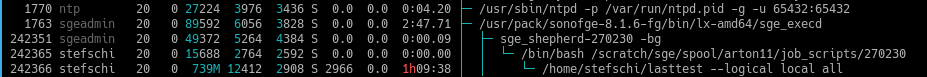
\includegraphics[width=14cm]{Screenshot_SGE_Call.png}
%\end{frame}
%
%\begin{frame}[fragile]{Master Slaves Konzept}
%Nutzen der Umgebungsvariablen \& des Shared Homes
%
%Datei: print.0.sge\_rs
%\begin{verbatim}
%127.0.0.1 ::1 129.132.67.78 fe80::21e:67ff:fe54:9068|arton01
%\end{verbatim}
%
%To the shell now!
%\end{frame}
%
%{
%\usebackgroundtemplate{\pgfuseimage{bgdark}}
%\section{Einige Fallstricke}
%}
%\begin{frame}[fragile]{TcpStream with SGE array jobs}
%X Instanzen erhalten Adressinformationen über die anderen Instanzen
%
%Frage: Wie viele Verbindungen wird jede Instanz öffnen?
%\begin{minted}{rust}
%peer_streams = map.values()
%    .filter(|s| s.is_some())
%    .map(|s| s.unwrap())
%    .map(|(addr, data_port)|
%        TcpStream::connect(
%            SocketAddr::new(addr, data_port)))
%    .filter(|s| s.is_ok())
%    .map(|s| s.unwrap())
%    .collect();
%\end{minted}
%\end{frame}

{
\usebackgroundtemplate{\pgfuseimage{bgdark}}
\section{Questions}
}

%{
%\usebackgroundtemplate{\pgfuseimage{bgdark}}
%\section{Workshop time}
%}


% ----------------------------------------------------------------- %

{
\setbeamertemplate{footline}{}
\pgfdeclareimage[width=\paperwidth]{bg}{background-inverted.pdf}
\usebackgroundtemplate{\pgfuseimage{bg}}
\begin{frame}[standout]
	\begin{centering}
	{\Huge Thank you for your attention!}\\
	{\normalsize Stefan Schindler @dns2utf8 }\\
  {\normalsize Happy hacking! Please ask questions! }\\
	{\footnotesize slides \& Examples: \url{https://github.com/dns2utf8/thread-pools-and-iterators}}\\
	\end{centering}
\end{frame}
}


% ----------------------------------------------------------------- %

\pgfdeclareimage[width=\paperwidth]{bg}{background.pdf}

\begin{frame}[fragile]{Why another language? - 0}
  \begin{itemize}
    \item It is hard to write safe and correct code.
    \item Even harder to write correct parallel code.
  \end{itemize}

\begin{minted}{C}
char *pi = "3.1415926f32";
while(1) {
    printf("Nth number? ");  err = scanf("%d", &nth);

    if (err == 0 || errno != 0) {
      printf("invalid entry\n");    while (getchar() != '\n');
      continue;
    }

    printf("Input: %d\n", nth);
    printf("Gewünschte Stelle: '%c'\n", pi[nth]);
}
\end{minted}
\end{frame}


\begin{frame}[fragile]{Why another language? - 1}
\begin{minted}{rust}
let pi = "3.1415926f32";
loop {
    print!("Nth number? ");
    io::stdout().flush().unwrap(); // force display on terminal
    let mut input = String::new();
    match io::stdin().read_line(&mut input) {
        Ok(_bytes_read) => {
            let nth: usize = input.trim().parse()
                                  .expect("invalid selection");
            println!("{}-th: '{:?}'", nth, pi.chars().nth(nth));
        }
        Err(error) => println!("error: {}", error),
    }
}
\end{minted}
\end{frame}


\end{document}
